The earliest learnings from the experiments have shown that the severe class imbalance is present and the model tends to predict mostly pure background --- black images. In order to overcome this an asymmetrical loss can be used during training. Similarly to a weighted loss for a classification problem with class imbalance issue present, a weighted loss for segmentation task can be introduced. In this case different pixels from the prediction will receive a different weight based on some criteria. Yet the use of weights cannot be easily defined for Pearson correlation coefficients, it is possible to use them with MSE loss, because weights coefficients there can be added directly in front of the squared difference between pixels. 
\begin{figure}[H]
	\begin{center}
		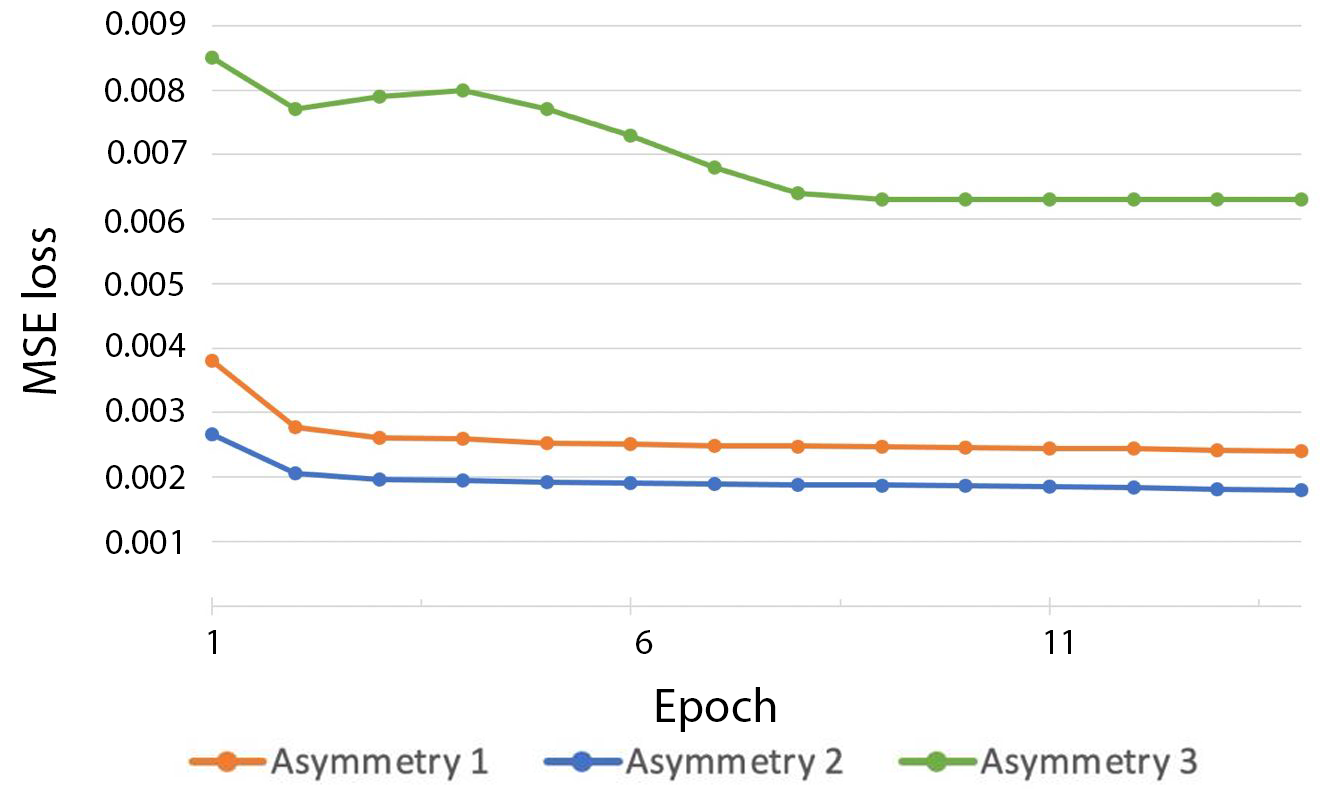
\includegraphics[width=0.5\linewidth]{bilder/golgi/asymmetrical-training.png}
		\caption{Punishing over and under predictions with asymmetrical MSE loss}\label{fig:golgi-asymmetrical-training}
	\end{center}
\end{figure}

Figure \ref{fig:golgi-asymmetrical-training} presents training learning curves from three asymmetrical approaches.

Asymmetry 2 is aimed to punish the errors on bright pixels more: when a model's pixel prediction is higher than a true one the loss will be higher. Yet this loss also encourages the model to underpredict and results in completely black images even though it has the lowest loss.
  \begin{lstlisting}
	  residual = prediction - ground_truth
	  loss = torch.where(residual < 0, residual ** 2, 2 * (residual) ** 2)
	  loss = torch.mean(loss)
	\end{lstlisting}

Asymmetry 1 is aimed to do the opposite and punish an underprediction: when a model's pixel prediction is lower than a true one the loss will be higher. This resulted in slightly brighter images
\begin{lstlisting}
	residual = prediction - ground_truth
	loss = torch.where(residual > 0, residual ** 2, 2 * (residual) ** 2)
	loss = torch.mean(loss)
  \end{lstlisting}

Asymmetry 3 is a stronger version of Asymmetry 1 and it results in 
	\begin{lstlisting}
		residual = prediction - ground_truth
		loss = torch.where(residual > 0, residual ** 3, 20 * (residual) ** 2)
		loss = torch.mean(loss)
	  \end{lstlisting}

All of the approaches above do not bring a significant change in the performance and a mostly black image remained to be an output. Interestingly, punishing underprediction has essentially backfired, as loss then supports an overprediction. Because setting the weights of one class to be smaller amounts to the same as setting the weights of the other class to be larger, and here as a result the model is more likely to overpredict. That is why the second asymmetry has a better loss, even though the logic behind it is not that obvious at first. 

There were other interesting approaches in asymmetrical losses tested that are depicted in Figure \ref{fig:golgi-asymmetrical-training}

1. Adjusting overall brightness. Leads the absence of bright spots and brightness gradients in the prediction. The illumination of the cell becomes uniform across all cells.
\begin{lstlisting}
	loss = loss +  prediction.sum() / ground_truth.sum()
  \end{lstlisting}

2. Adjusting overall brightness with a reversed division. Leads to fully white images as this would minimize the fraction in loss.
\begin{lstlisting}
	loss = loss + ground_truth.sum() / prediction.sum()
\end{lstlisting}

3. Multiplying loss with prediction will result in black images again, however multiplying with the ground truth yields more interesting results. However, the model is pushed to predict average gray color across the entire image for the most part.

\begin{lstlisting}
	loss = MSE(ground_truth, prediction)
	loss = torch.mul(loss, ground_truth)
\end{lstlisting}

4. Multiplying loss with 1 - ground\_truth also results in completely black images as such loss puts more puts more emphasis on the correct prediction of the background.
\begin{lstlisting}
	loss = MSE(ground_truth, prediction)
	loss = torch.mul(loss, 1 - ground_truth)
\end{lstlisting}

5. This improves the asymmetry approach 3, however now the highlighted regions simply include the whole cell.
\begin{lstlisting}
	loss = MSE(ground_truth, prediction)
	loss = torch.mul(loss, ground_truth) + ground_truth.sum() / prediction.sum()
\end{lstlisting}

6. Usual MSE.

7. Usual PCC.

From the experiments it became clear that the best approaches are PCC, pure MSE or MSE with the adjustment of overall brightness.

\begin{figure}[H]
	\begin{center}
		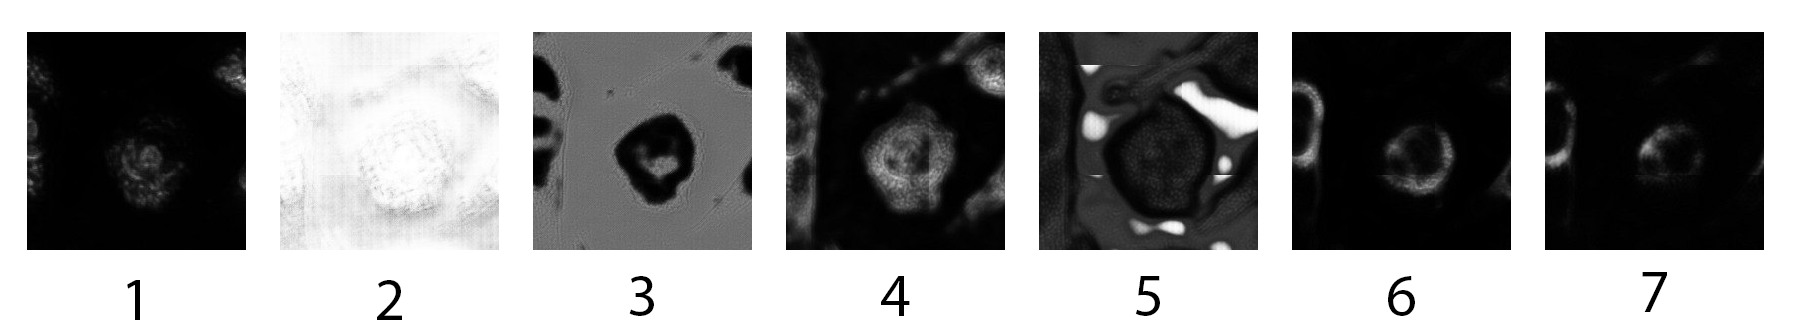
\includegraphics[width=\linewidth]{bilder/golgi/asymmetrical-predictions.png}
		\caption{Results of advanced versions of MSE training}\label{fig:golgi-asymmetrical-predictions}
	\end{center}
\end{figure} 